\chapter{Benchmark \& Discussion}

In this chapter the three algorithms are benchmarked with different parameters and scenarios. The first series of tests is conducted in a static environment for a basic understanding of the algorithm performance and the second series is held in various dynamic settings to explore the dynamic capabilities of the algorithms. The testing environment was the minion cluster of the departement of informatics at the University of Zurich. The cluster consists of 16 machines and each machine has 128 GB RAM and two E5-2680 v2 at 2.80GHz processors. Every processor has 10 cores and the interlink between the machines is a 40Gbps Infiniband setup. The cluster has different partition speeds (slow, fast, superfast). All tests were conducted on superfast partitions.

\section{Results I: Algorithms Performance in Static Environments}

- Problem Density
- Run Mode on Signal Collect

theoretical foundation: chapman benchmarking hybrid algorithms,!!! table, stuff

\subsection{Solution Quality over Time}

\subsection{Graph Structure}
\begin{figure}[H]
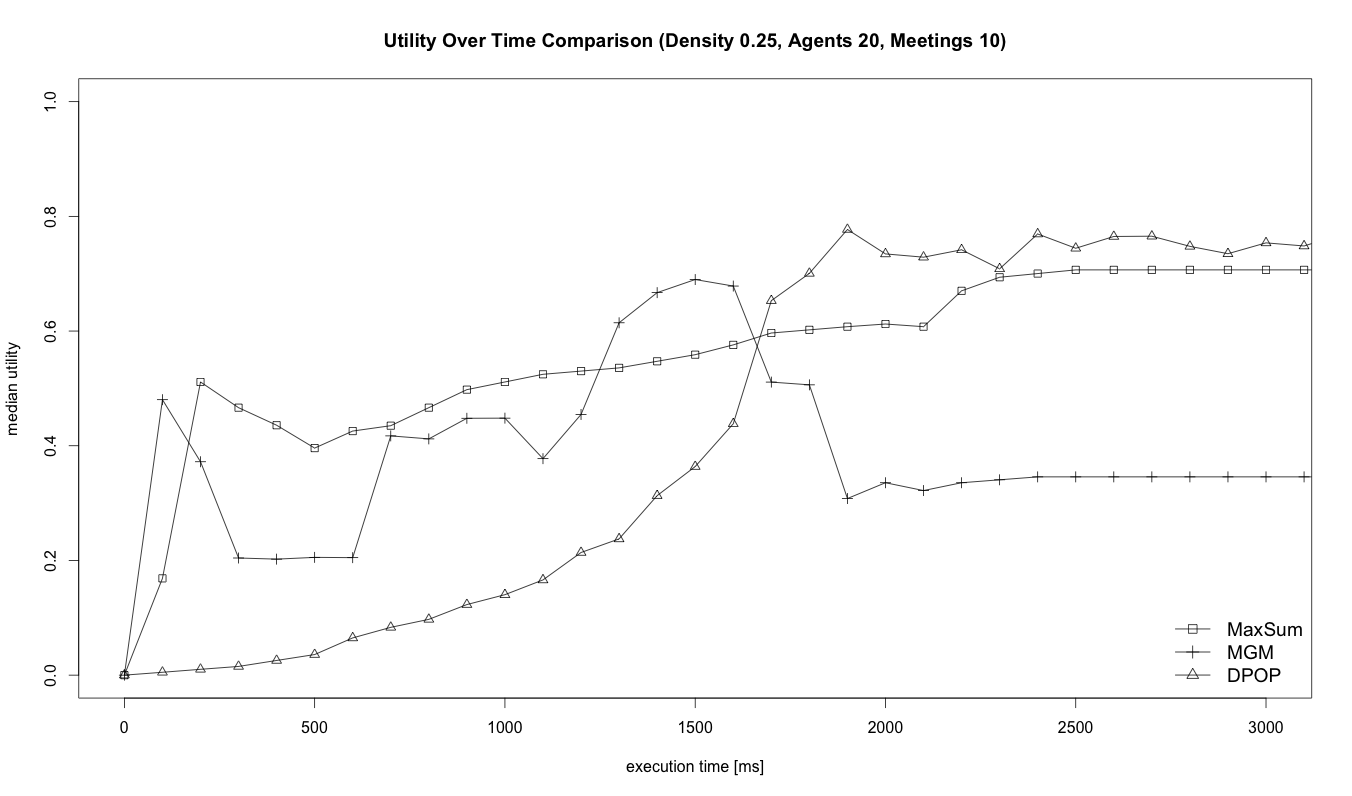
\includegraphics[width=400px]{graphics/experiments/static/quality/sq_1}
\centering
\caption{20/10, 0.25 density, all three, utility}
\label{fig:mgm_graph}
\end{figure}

\subsection{Graph Structure}
\begin{figure}[H]
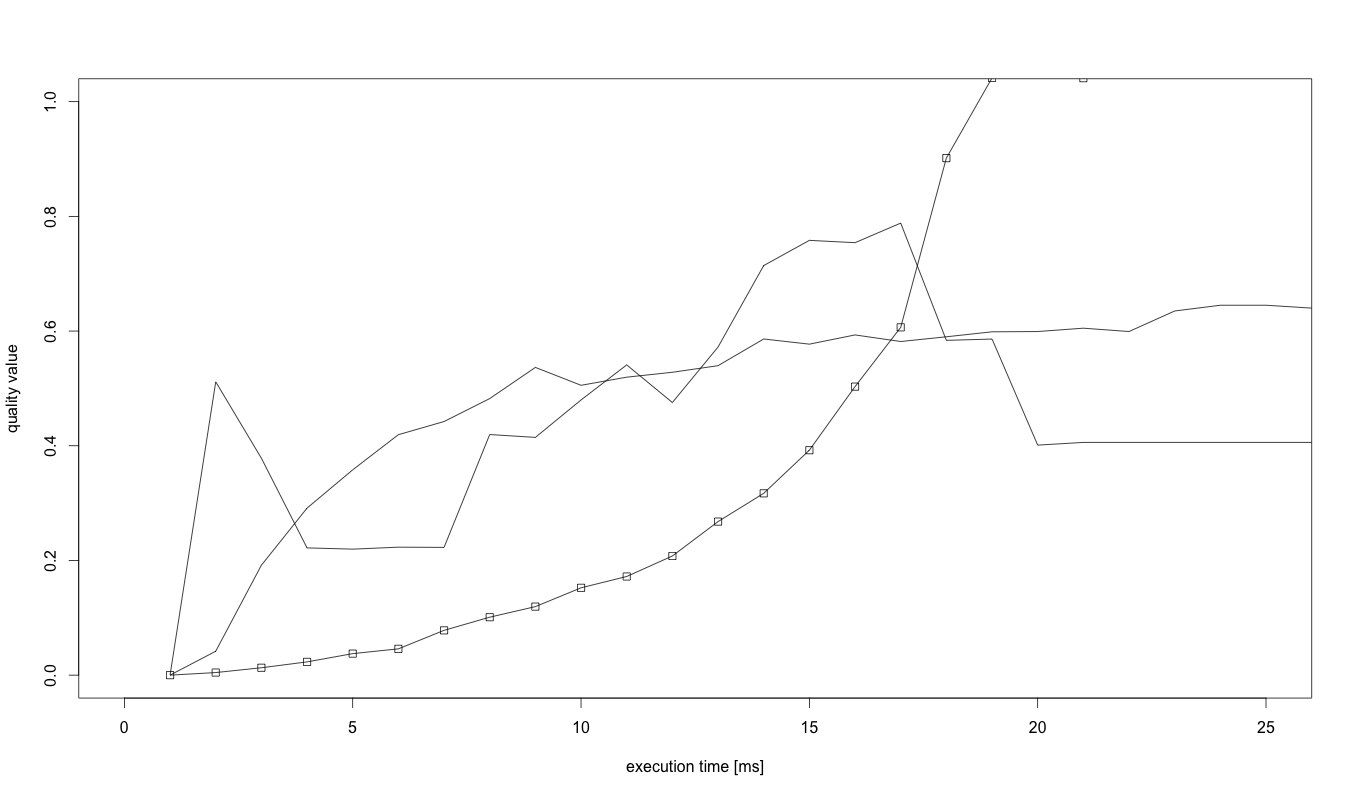
\includegraphics[width=400px]{graphics/experiments/static/quality/sq_2}
\centering
\caption{20/10, 0.25 density, all three, quality}
\label{fig:mgm_graph}
\end{figure}

\begin{table}[h]
\begin{tabular}{lllll}
10 &  &  &  &  \\
   &  &  &  &  \\
   &  &  &  &  \\
   &  &  &  & 
\end{tabular}
\caption{scale table}
\end{table}

%- Utility, Quality
%- Verlauf alle drei
%- Scalability: one, multiple machines
%- Quality Distribution

\subsection{Time to Convergence}

%\subsection{Conflicts over Time}
%- Verlauf alle drei
%- Scalability: one, multiple machines
%\subsection{Number of Messages}
%-  Verlauf alle drei
%- Scalability: one, multiple machines
%- Message Distribution

\begin{tabular}{llr}
\toprule
\multicolumn{2}{c}{Meetings Scalability (Asynchronous) \\
\cmidrule(r){1-4}
Meetings & MaxSum   & MGM & DPOP \\
\midrule
10 &        244.3     & 10.3 &	77.8\\
20  &     91.8	     & 4.4 & 63.7\\
30 &     70.7       	& 2.6 & 67.7\\
40 &     26.7     & 2.4 & 71\\
50 &     31.5     &	2.3 & 45\\

\begin{tabular}{llr}
\toprule
\multicolumn{2}{c}{Meetings Scalability (Synchronous) \\
\cmidrule(r){1-4}
Meetings & MaxSum   & MGM & DPOP \\
\midrule
10 & 31.1	 & 46.45 &	100.2\\
20  & 6.75	 & 38.7 & 91.5\\
30 & 2.6	& 33.8 & 63.25\\
40 & 2.3 & 34.65 & 57.85\\
50 & 2.3 & 23.95 &	67.3\\

\bottomrule
\end{tabular}

%- More time to find a valid solution -> could be local optima
%- Scalability: one, multiple machines
%- Convergence Distribution: how often does it converge -> dpop should always converge
%

\section{Results II: Algorithms Performance in Dynamic Environments}

%petcu 2007
%
%- Additional parameter
%- Different Scenarios: Constraints, Variables, Domain
%- Change one, multiple
%- Amount of Change: Percentage, Number
%
%- Number of Agents: 10,100,1000
%- Number of Meetings; 10,100, 1000
%- Number of Timeslots: 1000
%
%constraints: mode, interval, percentage
%variables: mode, interval, new Neighbourhood, new Agent, add / remove, how many
%domain: mode, interval, percentage, increase / decrease

\subsection{Stability}


\begin{tabular}{llr}
\toprule
\multicolumn{2}{c}{Item} \\
\cmidrule(r){1-2}
Animal    & Description & Price (\$) \\
\midrule
Gnat      & per gram    & 13.65      \\
          & each        & 0.01       \\
Gnu       & stuffed     & 92.50      \\
Emu       & stuffed     & 33.33      \\
Armadillo & frozen      & 8.99       \\
\bottomrule
\end{tabular}

%\cite{Verfaillie2005}
%
%%- Utility, Quality
%%- Multiple change: Peak Average
%%- Median Utility
%
%- Rate / Avg. Conflicts - Density!! Mailler2014, -> Definition Density einfügen

% dpop should not scale well, mgm should not

\subsection{Rebound Time}


%- utility, quality
%- Single change
%- Distribution
%- Verlauf alle drei
%- given timeframe -> lowest to highest avg.

% Please add the following required packages to your document preamble:

